\switchcolumn[1]*
\codeblock{kfac/scaffold}
\switchcolumn[0]

While KFAC has many nuances, its structure can be broken down into a general scaffold that simplifies its complexity into manageable sub-tasks.
At its core, KFAC approximates curvature matrices using a Kronecker-factorized structure, significantly reducing computational and memory costs.
In this section, we start from the general form of relevant curvature matrices, discuss how their structure enables a Kronecker-factored approximation, and introduce the core components of KFAC.
This scaffold---accompanied by the code snippets on the right---serves as the foundation for a systematic implementation, offering intuition on how Kronecker factors are computed and why such a decomposition is beneficial.
We keep the discussion general and highlight how to adapt the code to approximate any curvature matrix introduced in the previous section.
The next section will then focus on the specific case of KFAC for the generalized Gauss-Newton (GGN) of linear layers.

Many relevant matrices---such as the GGN, the type-I, the type-II, and the empirical Fisher---share a common structure
\begin{align*}
  \mC&(\vtheta^{(i)}) \\
  &= R \sum_n
  (\jac_{\vtheta^{(i)}} \vf_n)^{\top}
  \left[ \bullet(\vf_n, \vy_n) \right]
  (\jac_{\vtheta^{(i)}} \vf_n)\,
\end{align*}
where $\bullet \in \sR^{\gF \times \gF}$ is a positive semi-definite matrix in the prediction space that depends on the prediction $\vf_n$ and target $\vy_n$.
This term is sandwiched between the Jacobians of the network's prediction with respect to the parameters $\vtheta^{(i)}$ in layer $i$.
Directly computing and storing these matrices is often untractable, motivating approximation schemes such as KFAC.
The key idea behind KFAC is to exploit a Kronecker-product structure in the Jacobians $J_{\vtheta^{(i)}}(f_n)$ to approximate $\mC(\vtheta^{(i)})$ as
\begin{align*}
  \mC(\vtheta^{(i)})
  \approx
  \kfac(\mC(\vtheta^{(i)}))
  \coloneqq \mA^{(i)} \otimes \mB^{(i)}.
\end{align*}
For a composition of functions $$f \coloneqq f^{(L)} \circ f^{(L-1)} \circ \dots \circ f^{(1)}$$ with parameters $$\vtheta = \left[ \vtheta^{(1)}, \dots, \vtheta^{(L)} \right],$$ KFAC yields a block-diagonal approximation of the full curvature matrix $C(\vtheta)$, where each block corresponds to a layer and is of the form $\kfac(C(\vtheta^{(i)}))$.

In this approximation, $\mA^{(i)}$ is computed from the inputs to layer $i$, and we refer to it as \emph{input-based Kronecker factor}.
Similarly, $\mB^{(i)}$ is computed from gradients \wrt layer $i$'s output, and we call it the \emph{grad-output-based Kronecker factor}.

\subsection{Why use a Kronecker structure?}
Having a Kronecker structured approximation for $\mC(\vtheta^{(i)})$ has multiple advantages and motivations, that coincide well with the block diagonal structure.

\subsubsection{Memory and compuational efficiency}
\label{sec:mem_comp_eff_kron}
Most of the memory and computational gains of Kronecker factorization arise from the ability to express matrix operations on the dense representation
\begin{align*} \mA &\otimes \mB \\
=&\begin{bmatrix}
  a_{11} & \dots & a_{1n_2} \\
  \vdots & \ddots & \vdots \\
  a_{n_11} & \dots & a_{n_1n_2}
\end{bmatrix}
\otimes
\begin{bmatrix}
  b_{11} & \dots & b_{1m_2} \\
  \vdots & \ddots & \vdots \\
  b_{m_11} &  \dots & b_{m_1m_2}
\end{bmatrix} \\
=&\begin{bmatrix}
  a_{11} \mB & \dots & a_{1n_2} \mB \\
  \vdots & \ddots & \vdots \\
  a_{n_11} \mB & \dots & a_{n_1n_2} \mB
\end{bmatrix} \in \R^{n_1m_1 \times n_2m_2}
\end{align*}
in terms of operations on the individual factors $\mA$ and $\mB$.
This drastically reduces memory requirements, as we only need to store and handle these smaller matrices (\ie, $\mathcal{O}(n_1n_2 + m_1m_2)$) rather than the full Kronecker product (\ie $\mathcal{O}(n_1n_2m_1m_2)$). For key matrix operations, we have:

\paragraph{Matrix-vector product}
Let $\vv \in \R^{n_2m_2}$, then we have
$$ (\mA \otimes \mB) v = \text{vec}(\mA \mV \mB) $$
with $\mV \in \R^{n_2\times m_2}$ and $v \coloneqq \text{vec}(V)$.

\paragraph{Matrix transpose}
$$ (A \otimes B)^{\top} = A^{\top} \otimes B^{\top} $$

\paragraph{Matrix inverse}
$$ (A \otimes B)^{-1} = A^{-1} \otimes B^{-1} $$

\paragraph{Matrix mutliplication}
Let $\mC \in \R^{n_2 \times d_1}$ and $\mD \in \R^{m_2 \times d_2}$, then we have
$$ (\mA \otimes \mB)(\mC \otimes \mD) = \mA \mC \otimes \mB \mD. $$

\subsubsection{Naturally occuring structure}

The Kronecker strucutre in KFAC arises naturally in the expression for $\mC(\vtheta^{(i)})$ due to the structure of the layer Jacobians, providing a strong motivation for its use.
To see this, we start by rewriting $\mC(\theta^{(i)})$.
Since $\bullet(\vf_n, \vy_n)$ is a positive semi-definite matrix, it can be decomposed as a sum of outer products of $\dim(\gF)$ vectors: $$\bullet(\vf_n, \vy_n) = \sum_{c=1}^{\dim(\gF)} \blacktriangle_c(\vf_n, \vy_n) (\blacktriangle_c(\vf_n, \vy_n))^{\top}$$
where we define $\blacktriangle_{n,c} := \blacktriangle_c(\vf_n, \vy_n) \in \sR^{\gF}$.
Substituting this into the expression for the curvature matrix, we obtain:
\begin{align*}
  \mC(&\vtheta^{(i)}) \\
  =&
  R \sum_n \sum_{c}
  (\jac_{\vtheta^{(i)}} \vf_n)^{\top}
  \blacktriangle_{n,c} \blacktriangle_{n,c}^{\top}
  (\jac_{\vtheta^{(i)}} \vf_n)
\end{align*}
By applying the chain rule to split the Jacobian at the layer output $\vx^{(i)} = f^{(i)}(\vx^{(i-1)}, \vtheta^{(i)})$, we get
\begin{align*}
  (\jac_{\vtheta^{(i)}} \vf_n)^{\top}
  =
  (\jac_{\vtheta^{(i)}} \vx^{(i)}_n)^{\top}
  (\jac_{\vx_n^{(i)}} \vf_n)^{\top}.
\end{align*}
Substituting this back, the curvature matrix becomes
\begin{align*}
  \mC(\vtheta&^{(i)}) \\ =& R \sum_n \sum_{c}
  &&(\jac_{\vtheta^{(i)}} \vx^{(i)}_n)^{\top} \\
  & &&(\jac_{\vx_n^{(i)}} \vf_n)^{\top}
  \blacktriangle_{n,c}
  \blacktriangle_{n,c}^{\top}
  (\jac_{\vx_n^{(i)}} \vf_n) \\
  & &&(\jac_{\vtheta^{(i)}} \vx^{(i)}_n).
\end{align*}
The Kronecker structure emerges naturally in the output-parameter Jacobian $\jac_{\vtheta^{(i)}} \vx_n^{(i)}$ of a layer.
We have already seen this in the previous chapter, such as in the output-weight Jacobian of a linear layer, where the Kronecker structure arises explicitly (cf. \Cref{ex:linear_layer_jacobians}), with one of the Kronecker factors given by the layer input $\vx^{(i-1)}_n$.

Assuming a Kronecker-product structure of the form:
$$ a \otimes b := (\jac_{\vtheta^{(i)}} \vx^{(i)}_n)^{\top}
(\jac_{\vx_n^{(i)}} \vf_n)^{\top}
\blacktriangle_{n,c} $$
we can observe the following identity for each summand:
\begin{align*}
(a \otimes b)^T (a \otimes b) &= (b^T \otimes a^T)(a \otimes b) \\
&= a^Ta \otimes b^Tb
\end{align*}
which follows directly from the properties of the Kronecker product (cf.~\Cref{sec:mem_comp_eff_kron}).

The primary approximation in KFAC is then how to efficiently resolve the summation over $n$ and $c$ in the above expression---known as KFAC's expectation approximation (cf.~\Cref{def:kfac_exp_approx})---and how to generalize this structure to more complex layers.

\subsubsection{Input-based and grad-output-based Kronecker factors}
The derivation above also motivates why KFAC results in two distinct Kronecker factors: one based on layer inputs ($\mA^{(i)}$) and the other based on gradients with respect to the layer ouput ($\mB^{(i)}$). Specifcally, we can interpret $(\jac_{\vtheta^{(i)}} \vx_n^{(i)})^{\top} \blacktriangle_{n,c}$ as a \emph{pseudo-gradient}. In fact, setting
$$\blacktriangle_{n,c} \leftarrow \nabla_{\vf_n} c(\vf_n, \vy_n)\,$$
we obtain
$$(\jac_{\vtheta^{(i)}} \vx_n^{(i)})^{\top} \blacktriangle_{n,c} = \nabla_{\vx_n^{(i)}} c(\vf_n, \vy_n),$$
which is the per-datum loss gradient with respect to layer $i$'s output.
In summary, we identify the following dependencies of the Kronecker factors $\mA^{(i)}$ and $\mB^{(i)}$, justifying their names:
\begin{align*}
  \mA^{(i)} &= \mA^{(i)}( \{\vx_{n}^{(i-1)}\}_n ),
  \\
  \mB^{(i)} &= \mB^{(i)}( \{ (\jac_{\vx_n^{(i)}}\vf_{n})^{\top} \blacktriangle_{n,c}\}_{n,c}).
\end{align*}

\subsection{Algorithmic outline}

From the previous section, we already gained an overview of the shared structure of KFAC across different curvature approximations, with the primary variation arising in the grad-output-based Kronecker factors.
Here, we summarize the common computational scaffold, with the accompanying code snippet implementing the shared computations (Steps 1 and 2).
A complete example derivation, including Steps 3–5, is provided in the next section for the Generalized Gauss-Newton (GGN) together with potential test cases to verify the implementation numerically (cf. \Cref{sec:kfac-expand-linear}).

\paragraph{Step 1:} Perform a forward pass to compute $\{\vf_n\}_n $, storing the layer inputs $\{\vx_n^{(i-1)} \}_n$ and outputs $\{\vx_n^{(i)}\}_n$ of all layers $i$ for which a KFAC approximation is defined.

\paragraph{Step 2:} Compute the input-based Kronecker factors $\mA^{(i)}$ using the layer inputs $\{\vx_n^{(i-1)}\}_n$ taking into account the KFAC variation that is desired.

\paragraph{Step 3:} Generate the vectors $\{\blacktriangle_{n,c}\}_{n,c}$ to be backpropagated, taking into account the specified KFAC approximation. Compute the pseudo-gradients $\{(\jac_{\vx_n^{(i)}} \vf_n)^{\top} \blacktriangle_{n,c} \}_{n,c}$ \wrt the layer outputs. Finally, compute the output-based Kronecker factors $\mB^{(i)}$.%\footnote{If no backpropagated vectors are produced, simply set $\mB^{(i)} = \mI$.}

\paragraph{Step 4:} Account for scaling caused by the loss function's reduction $R$.

\paragraph{Step 5:} Return the KFAC approximation in the form $\mA^{(i)}, \mB^{(i)}$ for all supported $i$.

\switchcolumn[1]*
\codeblock{kfac/backpropagated_vectors}
\switchcolumn[0]

\subsection{Backpropagated Vectors}
The computational scaffold can be flexibly adapted to various curvature matrices by modifying the choice of backpropageted vectors $\blacktriangle_{n,c}$ and the reduction factor $R$. Below, we summarize the different curvature definitions and their associated backpropagated vectors. For further background on each curvature, refer to Chapter 2.\footnote{Input-only: Two concurrent works have recently proposed to completely remove the backpropagations of KFAC to compute $\mB^{(i)}$, and instead set $\mB^{(i)} = \mI$. In this case, we do not need to generate vectors for backpropagation.
}

\paragraph{Generalized-Gauss Newton (GGN)}
The GGN is given by\begin{align*}
\ggn_{\vtheta}&\gL_{\sD}(\vtheta) \\
&= R \sum_{n=1}^N
  \left[\jac_{\vtheta} \vf_n\right]^{\top}
  \left[\hess_{\vf_n} c(\vf_n, \vy_n)
  \right]
  \left[\jac_{\vtheta} \vf_n\right].
\end{align*}
Using the symmetric decomposition
$$\mS_n \mS_n^{\top} = \hess_{\vf_n} c(\vf_n, \vy_n),$$ we identify for the backprograted vector
\begin{align*}
  \blacktriangle_{n,c} = [\mS_n]_{:,c}.
\end{align*}
Thus, we end up backpropagating each column of the Hessian decomposition $\mS_n$, introducing $\dim(\gF)$ backpropagations, each of which is roughly as expensive as computing a parameter gradient.

\paragraph{Type-II Fisher}
For convex loss functions, the Type-II Fisher curvature matrix coincides with the GGN. It is defined as
\begin{align*}
\fisher^{\text{II}}_{\vtheta} \gL_{\sD}(\vtheta) = \lim_{M \to \infty} \frac{R}{M} \sum_{n=1}^N & \left(\jac_{\vtheta} \vf_n\right)^{\top} \\
&\hess_{\vf_n} c(\vf_n, \tilde{\vy}_{n,m}) \\
&\jac_{\vtheta} \vf_n.
\end{align*}
Using the same decomposition as in the GGN case, we obtain:
\begin{align*}
  \blacktriangle_{n,c} = [\mS_n]_{:,c}.
\end{align*}

\paragraph{MC-sampled Type-I Fisher}
The Type-I Fisher, approximated via Monte Carlo (MC) sampling, is given by:
\begin{align*}
&\fisher^{\text{I}}_{\vtheta}\gL_{\sD}(\vtheta) \\
&\begin{aligned}
= \lim_{M \to \infty} \frac{R}{M} \sum_{n=1}^N
  &\left( \jac_{\vtheta} \vf_n\right)^{\top} \\
  &
\begin{aligned}
  \big[ 
  &\nabla_{\vf_n} c(\vf_n, \tilde{\vy}_{n,m}) \\
  &\nabla_{\vf_n} c(\vf_n, \tilde{\vy}_{n,m})^{\top}
  \big] 
\end{aligned} \\
  &\jac_{\vtheta} \vf_n.
\end{aligned}
\end{align*}
By a similar derivation, this leads to the pseudo-gradient
\begin{align*}
  \blacktriangle_{n,m}
  %&= -\nabla_{\vf_n} \log r(\rvy=\tilde{\vy}_{n,m} \mid \rvf = \vf_n)
  %\\
  &= \nabla_{\vf_n}  c(\vf_n, \tilde{\vy}_{n,m})
\end{align*}
where $\tilde{\vy}_{n,m} \stackrel{\text{\iid}}{\sim} r(\rvy \mid \vf = \vf_n)$ is a sample from the model's predictive distribution (see \Cref{sec:fisher} for a reminder).
The number of Monte Carlo samples, $M$, controls the number of backpropgations:
\begin{itemize}
 \item For \emph{computational efficiency}, choosing $M~<~\dim(\gF)$ makes sense becuause this reduces the number of backpropagations from $\dim(\gF)$ (as in the Type-II case) to $M$.
 \item For \emph{practical settings} $M$ is usually set to $1$ to save computation.
 \item For \emph{verification}, a larger $M$ can be used to ensure convergence to the expected value.
\end{itemize}

\paragraph{Empirical Fisher}
The empirical Fisher replaces the expectation approximation in the Type-I Fisher with a single-sample estimate:
\begin{align*}
  \fisher_\vtheta^{\text{emp}} &\gL_{\sD}(\vtheta) \\
  &\begin{aligned}= R \sum_{n=1}^N
      &\jac_{\vtheta} \vf_n^{\top} \\
      & \nabla_{\vf_n} c(\vf_n, \tilde{\vy}_{n}) (\nabla_{\vf_n} c(\vf_n, \tilde{\vy}_n ))^{\top} \\
      &\jac_{\vtheta} \vf_n.
  \end{aligned}
\end{align*}
The pseudo-gradient reduces then to
\begin{align*}
  \blacktriangle_{n,1}
  % &= -\nabla_{\vf_n} \log r(\rvy=\vy_n \mid \rvf = \vf_n)
  % \\
  &= \nabla_{\vf_n}  c(\vf_n, \vy_n).
\end{align*}
This is essentially the same target as when computing the empirical risk, which means we can compute the corresponding KFAC approximation by re-cycling the backward pass from the gradient computation.

% \item Input-only: Two concurrent works have recently proposed to completely remove the backpropagations of KFAC to compute $\mB^{(i)}$, and instead set $\mB^{(i)} = \mI$.
%   In this case, we do not need to generate vectors for backpropagation.

\begin{figure}[t!]
  \centering
  \begin{minipage}[t]{0.485\linewidth}
    \centering
    \textbf{FULL}
  \end{minipage}
  \hfill
  \begin{minipage}[t]{0.485\linewidth}
    \centering
    \textbf{KFAC}
  \end{minipage}
  \\
  \begin{minipage}[t]{0.485\linewidth}
    \centering
     GGN ($\cvec$)\vspace{1ex}
    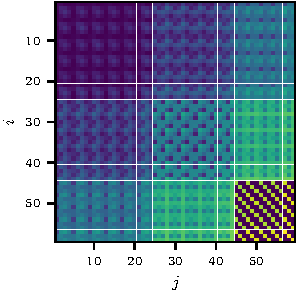
\includegraphics[width=0.8\linewidth]{../kfs/plots/synthetic_cvec_ggn_full.pdf}
  \end{minipage}
  \hfill
  \begin{minipage}[t]{0.485\linewidth}
    \centering
    GGN ($\cvec$)\vspace{1ex}
    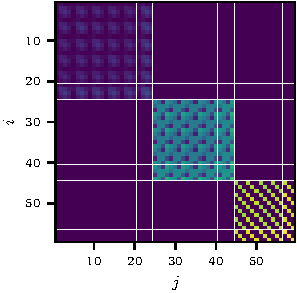
\includegraphics[width=0.8\linewidth]{../kfs/plots/synthetic_cvec_ggn_kfac.pdf}
  \end{minipage}
  \\
  \begin{minipage}[t]{0.485\linewidth}
    \centering
     GGN ($\rvec$)\vspace{1ex}
    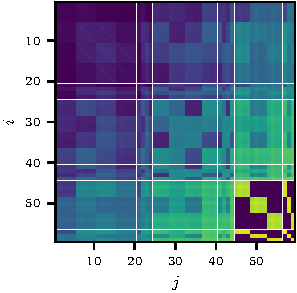
\includegraphics[width=0.8\linewidth]{../kfs/plots/synthetic_rvec_ggn_full.pdf}
  \end{minipage}
  \hfill
  \begin{minipage}[t]{0.485\linewidth}
    \centering
    GGN ($\rvec$)\vspace{1ex}
    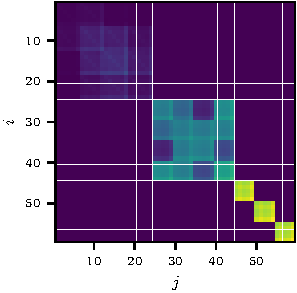
\includegraphics[width=0.8\linewidth]{../kfs/plots/synthetic_rvec_ggn_kfac.pdf}
  \end{minipage}
  \\
  \begin{minipage}[t]{0.485\linewidth}
    \centering
    MC-Fisher ($\cvec$)\vspace{1ex}
    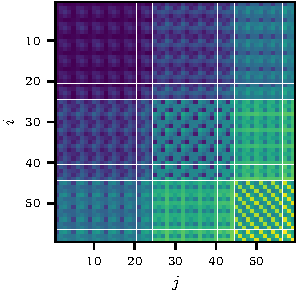
\includegraphics[width=0.8\linewidth]{../kfs/plots/synthetic_cvec_mcfisher_100_full.pdf}
  \end{minipage}
  \hfill
  \begin{minipage}[t]{0.485\linewidth}
    \centering
    MC-Fisher ($\cvec$)\vspace{1ex}
    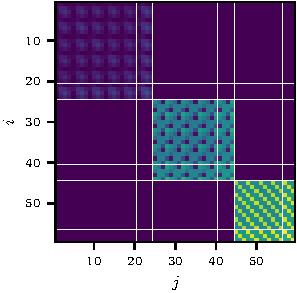
\includegraphics[width=0.8\linewidth]{../kfs/plots/synthetic_cvec_mcfisher_100_kfac.pdf}
  \end{minipage}
  \\
  \begin{minipage}[t]{0.485\linewidth}
    \centering
    MC-Fisher ($\rvec$)\vspace{1ex}
    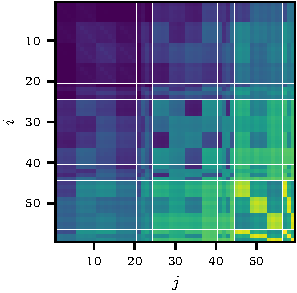
\includegraphics[width=0.8\linewidth]{../kfs/plots/synthetic_rvec_mcfisher_100_full.pdf}
  \end{minipage}
  \hfill
  \begin{minipage}[t]{0.485\linewidth}
    \centering
    MC-Fisher ($\rvec$)\vspace{1ex}
    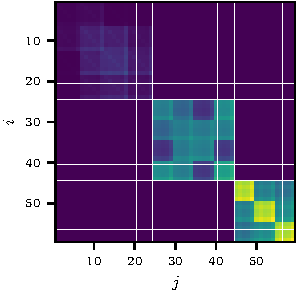
\includegraphics[width=0.8\linewidth]{../kfs/plots/synthetic_rvec_mcfisher_100_kfac.pdf}
  \end{minipage}
  \\  
  \begin{minipage}[t]{0.485\linewidth}
    \centering
    Emp-Fisher ($\cvec$)\vspace{1ex}
    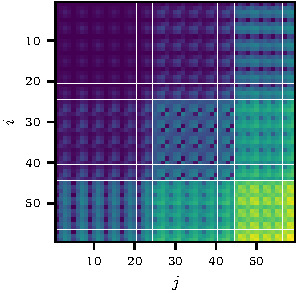
\includegraphics[width=0.8\linewidth]{../kfs/plots/synthetic_cvec_empfisher_full.pdf}
  \end{minipage}
  \hfill
  \begin{minipage}[t]{0.485\linewidth}
    \centering
    Emp-Fisher ($\cvec$)\vspace{1ex}
    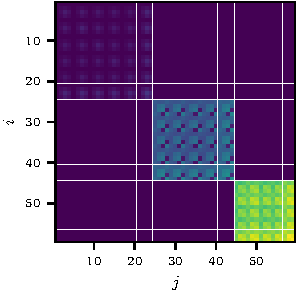
\includegraphics[width=0.8\linewidth]{../kfs/plots/synthetic_cvec_empfisher_kfac.pdf}
  \end{minipage}
  \\
  \begin{minipage}[t]{0.485\linewidth}
    \centering
    Emp-Fisher ($\rvec$)\vspace{1ex}
    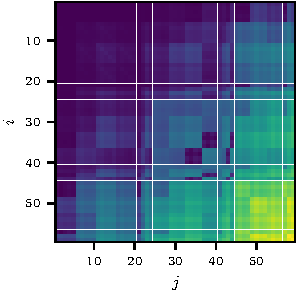
\includegraphics[width=0.8\linewidth]{../kfs/plots/synthetic_rvec_empfisher_full.pdf}
  \end{minipage}
  \hfill
  \begin{minipage}[t]{0.485\linewidth}
    \centering
    Emp-Fisher ($\rvec$)\vspace{1ex}
    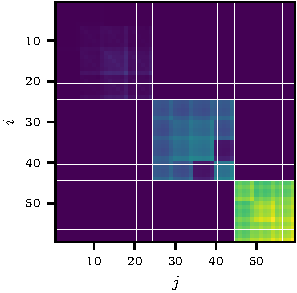
\includegraphics[width=0.8\linewidth]{../kfs/plots/synthetic_rvec_empfisher_kfac.pdf}
  \end{minipage}
    \caption{Visualization of full curvatures (GGN, MC-sampled Fisher and Empirical Fisher) and their corresponding KFAC approximation using different flattening schemes. All curvatures were evaluated on synthetic data ($N = 100$) using an MLP with three fully-connected layers and ReLU activations (5-4-4-3, our notation considers applying the weight matrix and adding the bias as two layers, hence $L=6$) and square loss. For the MC-sampled Fisher we consider $M = 100$ Monte Carlo samples. This follows the setup in \Cref{fig:hessian-block-structure}.
    Plots produced with \repofile{plots/synthetic_kfac}.}
    \label{fig:kfac-full-comparison}
\end{figure}

%%% Local Variables:
%%% mode: latex
%%% TeX-master: "../main"
%%% End:
